\documentclass[10pt, handout]{beamer} % mathserif for normal math fonts.

\usefonttheme[onlymath]{serif}
\usepackage{amsmath,mathtools}
\usepackage{calc}
\usepackage{caption}
\usepackage{color}

% KRJ: Removed because of xelatex
%\usepackage[EU1]{fontenc}
\usepackage[utf8]{inputenc}
\usepackage{lmodern}
\usepackage[english]{babel}
\usepackage[babel]{csquotes}

% KRJ: xelatex stuff
%\usepackage{xltxtra}
%\usepackage{polyglossia}
%\usepackage{fontspec}
%\usepackage[]{unicode-math}
%\setmainfont{XITS}
%\setmathfont{XITS Math}
%\usepackage{csquotes}

\usepackage{subcaption}
\usepackage{listings}
\usepackage[style=verbose]{biblatex}
\lstset{ %
language=Python,     
basicstyle=\tiny,   
numbers=none,         
numberstyle=\tiny,    
stepnumber=1,         
numbersep=5pt,        
backgroundcolor=\color[gray]{0.95},  
showspaces=false,               
showstringspaces=false,       
showtabs=false,             
frame=single,        
tabsize=2,         
captionpos=b,      
breaklines=break,  
linewidth=0.98\linewidth,
xleftmargin=0.0\linewidth,
breakatwhitespace=false,   
%escapeinside={\%}{)}     
    identifierstyle=\ttfamily,
    keywordstyle=\color[rgb]{0,0,1},
    commentstyle=\color[rgb]{0.133,0.545,0.133},
    stringstyle=\color[rgb]{0.627,0.126,0.941}
}

\usetheme[titleflower=true]{chalmers} % titleflower = true or false

\title{Modelling of electrokinetic flow using the lattice-Boltzmann
  method}

\subtitle{Master's thesis presentation} % optional

\author[A. B\"ulling]{Andreas B\"ulling} % [short
                                         % author(optional)]{many
                                         % authors}

\institute{Chalmers University of Technology} 

\date{December 20, 2012}

\footer{\insertshortauthor, Master's thesis presentation}

%\addbibresource{/home/klas/Documents/PhD/Library/Sources.bib}
%\let\oldfootnotesize\footnotesize
%\renewcommand*{\footnotesize}{\oldfootnotesize\tiny}
%\newcommand{\KRJScale}{0.33}

%\usepackage{../styles/KJCommands}

% KRJ, Colorbox for equations and theorems
%\usepackage[listings,theorems]{tcolorbox}
%\newenvironment{krjbox}[1]{
%\centering
%\tcolorbox[width=0.9\textwidth,colback=chalmersblue!5,colframe=chalmersblue,title=#1,fontupper=\scriptsize]}
%{\endtcolorbox}

\AtBeginSection[]
{
\begin{frame}
%\usebeamerfont{section title}\insertsection
\begin{columns}
\begin{column}[]{0.5\textwidth}
%\begin{center}
\vbox to .8\textheight{
\huge\bf\insertsection
\\[5cm]\vfill
}
%\end{center}
\end{column}
\begin{column}[b]{0.5\textwidth}
\vbox to .3\textheight{
\small{\tableofcontents[currentsection]}
\vfill
}
\end{column}
\end{columns}
\end{frame}
}

%\AtBeginSection[]{
%  \setbeamercolor{section in toc shaded}{use=structure,fg=structure.fg}
%  \setbeamercolor{section in toc}{fg=chalmersblue}
%  \setbeamercolor{subsection in toc shaded}{fg=black}
%  \setbeamercolor{subsection in toc}{fg=chalmersblue}
%  \frame<beamer>{
%  %\begin{multicols}{2}
%      \frametitle{Outline}
%      \setcounter{tocdepth}{1}  
%      \LARGE{
%        \tableofcontents[currentsection]
%      }
%  %\end{multicols} 
%  }
%}

% Notes in the document
%\setbeameroption{show notes} 

\newlength{\parskipbackup}
\setlength{\parskipbackup}{\parskip}
\newlength{\parindentbackup}
\setlength{\parindentbackup}{\parindent}

\let\notebackup\note
\renewcommand{\note}[1]{\notebackup{%
\mode<handout>{\addtocounter{page}{-1}}%
\setlength{\parindent}{0ex}%
\setlength{\parskip}{10pt}%
\noindent%
{\normalsize{}#1}%
\setlength{\parskip}{\parskipbackup}%
\setlength{\parindent}{\parindentbackup}%
}%
}

\newenvironment{itemize*}%
  {\begin{itemize}[<+->]%
\setlength{\itemsep}{2em}}%
    %\setlength{\parskip}{115pt}}%
  {\end{itemize}}

%def of various quantities

\newcommand{\J}{\ensuremath{\mathbf{J}}}
\newcommand{\C}{\ensuremath{\mathrm{c}}} 
\newcommand{\rhorm}{\ensuremath{\mathrm{\rho}}} 
\newcommand{\drm}{\ensuremath{\mathrm{d}}} 
\newcommand{\Prm}{\ensuremath{\mathrm{P}}} 
\newcommand{\ux}{\ensuremath{\mathrm{u_x}}} 
\newcommand{\uy}{\ensuremath{\mathrm{u_y}}} 
\newcommand{\Rerm}{\ensuremath{\mathrm{Re}}}
\newcommand{\Pe}{\ensuremath{\mathrm{Pe}}} 
\newcommand{\psirm}{\ensuremath{\mathrm{\psi}}} 
\newcommand{\R}{\ensuremath{\mathrm{R}}} 
\newcommand{\Gi}{\ensuremath{\mathrm{G_i}}} 

\newcommand{\ubf}{\ensuremath{\mathbf{u}}}
\newcommand{\ubar}{\ensuremath{\mathbf{\bar{u}}}}
\newcommand{\x}{\ensuremath{\mathbf{x}}}
\newcommand{\n}{\ensuremath{\mathbf{n}}}
\newcommand{\Q}{\ensuremath{\mathbf{Q}}}
\newcommand{\F}{\ensuremath{\mathbf{F}}}
\newcommand{\E}{\ensuremath{\mathbf{E}}}
\newcommand{\jj}{\ensuremath{\mathbf{j}}}
\newcommand{\cbf}{\ensuremath{\mathbf{c}}}
\newcommand{\ci}{\ensuremath{\mathbf{c}_i}}
\newcommand{\p}{\ensuremath{\mathbf{p}}}

\newcommand{\feq}{\ensuremath{f_i^{(eq)}}}
\newcommand{\feqe}[1]{\ensuremath{f_i^{(eq, #1)}}}
\newcommand{\fii}{\ensuremath{f_i}}
\newcommand{\fie}[1]{\ensuremath{f_i^{(#1)}}}
\newcommand{\rhoe}[1]{\ensuremath{\rho^{(#1)}}}
\newcommand{\Rexp}[1]{\ensuremath{\mathrm{\R}^{(#1)}}}
\newcommand{\Gie}[1]{\ensuremath{\mathrm{G_i}^{(#1)}}}
\newcommand{\je}[1]{\ensuremath{\mathbf{j}^{(#1)}}}
\newcommand{\ubare}[1]{\ensuremath{\mathbf{\bar{u}}^{(#1)}}}
\newcommand{\ue}[1]{\ensuremath{\mathbf{u}^{(#1)}}}
\newcommand{\ep}{\ensuremath{\epsilon}}
\newcommand{\pd}{\ensuremath{\ci\cdot\nabla}}
\newcommand{\bigO}[1]{\ensuremath{\mathcal{O}(#1)}}
\newcommand{\parti}[1]{\ensuremath{\partial_{#1}}}
\newcommand{\cc}[1]{\ensuremath{c_{i#1}}}
\newcommand{\uc}[1]{\ensuremath{u_{#1}^{(1)}}}
\newcommand{\dd}[2]{\ensuremath{\delta_{#1#2}}}
\newcommand{\deltasec}{\ensuremath{\dd{\alpha}{\beta}\dd{\gamma}{\delta}+
    \dd{\alpha}{\gamma}\dd{\beta}{\delta}
    +\dd{\alpha}{\delta}\dd{\beta}{\gamma}}}
\newcommand{\dab}{\ensuremath{\dd{\alpha}{\beta}}}


\newcommand{\todo}[1]{
\begin{center}\textcolor{red}{ \bf{TODO: #1}}\end{center}}



\begin{document}

\begin{frame}[plain]
  \titlepage
\end{frame}

\begin{frame}{Outline}
  \tableofcontents[pausesections]
\end{frame}

\section{Background}

\begin{frame}{Background}

%\setbeamercovered{transparent=50}
%\setbeamercovered{transparent}

\begin{itemize*}
\item Demand from both industry and academy on accurate modelling of
  electrokinetic systems.
\item Example of applications: drugs, biological chips, fuel cells...
\item A lattice-Boltzmann code is developed at Chalmers to deal with
  transport through complicated structures.
\item This work aims to investigate how electric effects may be integrated.
\end{itemize*}


\end{frame}

\begin{frame}[plain]
\begin{figure}
\begin{center}
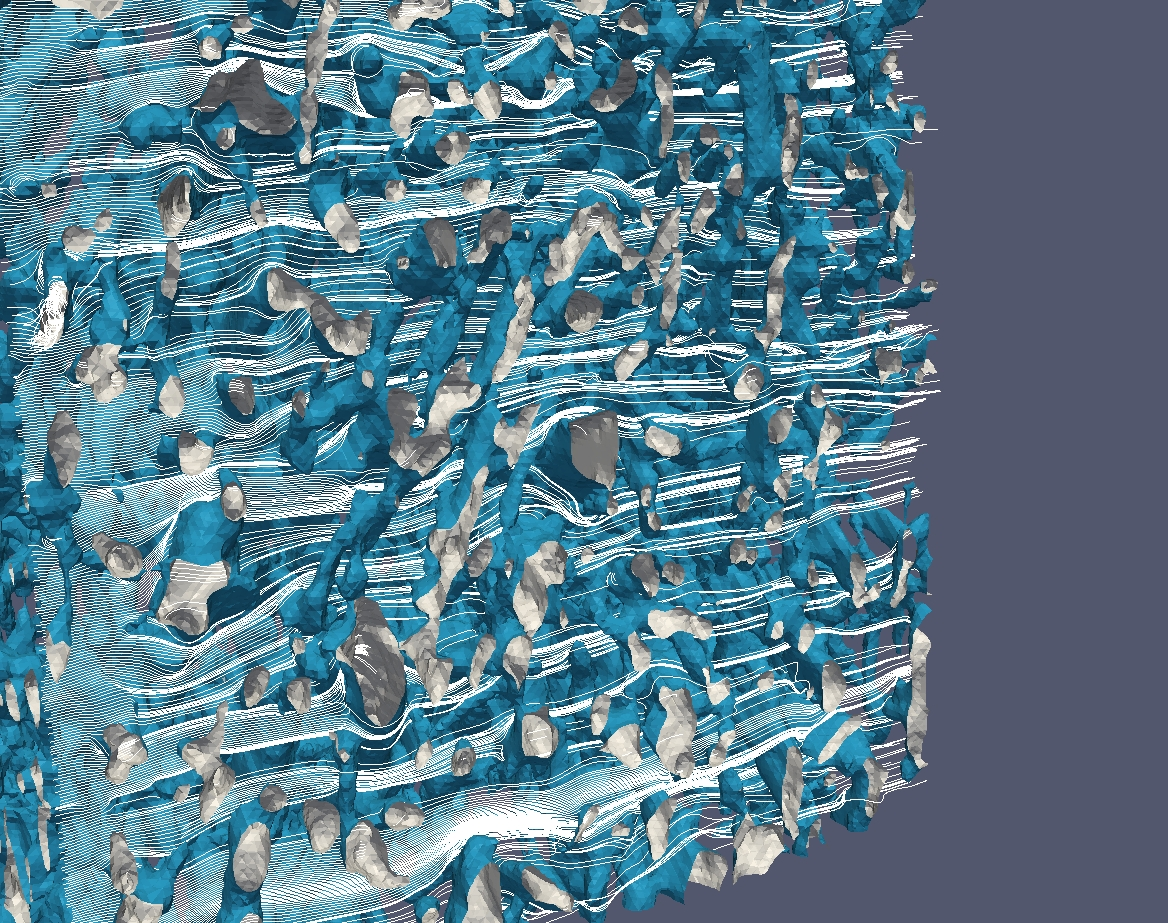
\includegraphics[width=1.0\textwidth]{fig/diffusion_w4.jpg}
\end{center}
%\caption{Visualisation of the coupling between the three equations
%  present in the model. Poisson's equation (PE), The set of
%  Nernst-Planck equations (NP$_1$ ... NP$_n$) for the different ion
%  species and the Navier-Stokes equations (NS). The dependencies have
%  also be marked with arrows indicating what quantities for a certain
%  equation that are needed from an other.}
%\label{fig:coupling}
\end{figure}
\end{frame}


\section{Electrokinetics}

\subsection{Basic concepts}

\begin{frame}{Sample system - a 2D channel}
Example of a ``simple'' electrokinetic system:

\begin{figure}
\begin{center}
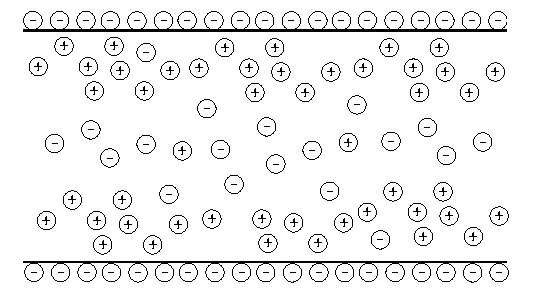
\includegraphics[width=0.7\textwidth]{../fig/channel.pdf}
\end{center}
\end{figure}

The solution contains charges, the walls are charged, external
electric/force fields may be present...

\end{frame}

\begin{frame}{Electrical double layers (EDLs)}
Ionic solution in contact with a charged object $\implies$ EDL

\begin{figure}
\begin{center}
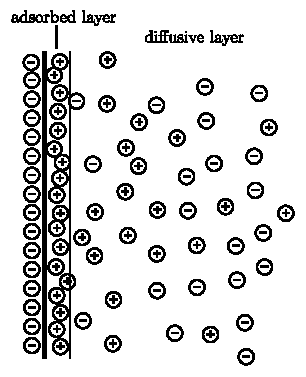
\includegraphics[width=0.5\textwidth]{../fig/edl.pdf}
\end{center}
\end{figure}

\end{frame}

\subsection{Modelling approach}

\begin{frame}{Involved equations}

\begin{itemize*}

\item The electric potential from the charge presence. Poisson's
  equation for electrostatics:
\begin{equation}\label{eq:pb}
\nabla^2\psirm = -\frac{\rho_e}{\epsilon_r \epsilon_0}
\end{equation}


\item The transport of charges due to diffusion, advection and the
  presence of electric fields. The Nernst-Planck equation:
\begin{equation}\label{eq:et:np}
\dfrac{\partial \C}{\partial t} = \nabla \cdot \left [
 D\nabla \C - \C\ubf + \frac{zq_eD}{k_BT}\C\nabla\psirm
\right]
\end{equation}

\item The flow field, affected by electrokinetic
  effects. (Incompressible) Navier-Stokes equations:
\begin{equation}\label{eq:et:ns_incompressible}
 \nabla \cdot \ubf = 0
\end{equation}
and

\begin{equation}\label{eq:et:ns_mom}
\rhorm \left (\dfrac{\partial \ubf}{\partial t} +
  \ubf \cdot \nabla \ubf 
  \right ) = - \nabla \Prm  + \mu \nabla^2 \ubf + \F
\end{equation}


\end{itemize*}

\end{frame}

\begin{frame}
\begin{figure}
\begin{center}
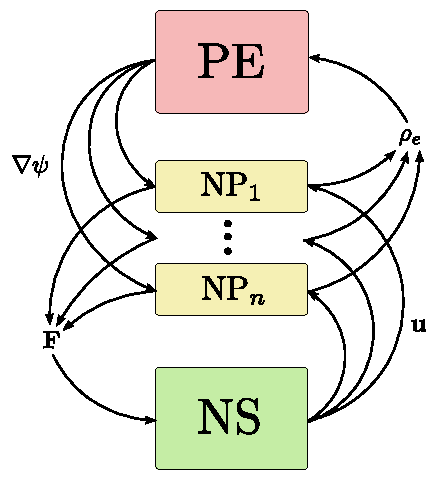
\includegraphics[width=0.5\textwidth]{../fig/coupling.pdf}
\end{center}
\caption{Visualisation of the coupling between the three equations
  present in the model. Poisson's equation (PE), The set of
  Nernst-Planck equations (NP$_1$ ... NP$_n$) for the different ion
  species and the Navier-Stokes equations (NS). The dependencies have
  also be marked with arrows indicating what quantities for a certain
  equation that are needed from an other.}
\label{fig:coupling}
\end{figure}
\end{frame}

\subsection{Some electrokinetic phenomena}

\begin{frame}{The electroviscous effect}

\begin{equation}
\J = -  \sigma \nabla \phi  
\end{equation}

\begin{equation}
\F = - \rho_e \nabla \phi
\end{equation}

\begin{figure}
\begin{center}
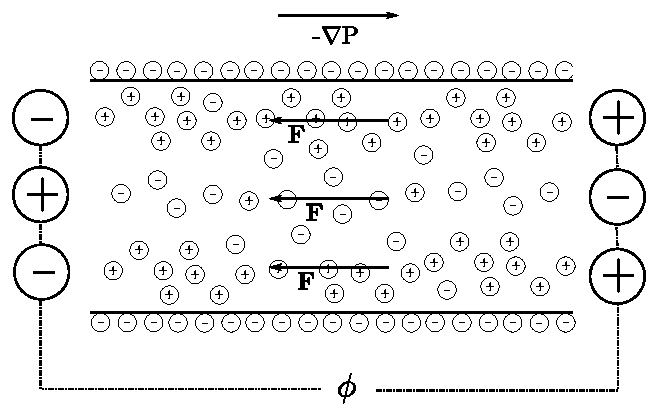
\includegraphics[width=0.7\textwidth]{../fig/channel_electroviscous.pdf}\\
Streaming potential
\end{center}
\end{figure}

\end{frame}

\begin{frame}{Electroosmosis}

\begin{equation}
\F = \rhorm_e \E_{ext}
\end{equation}

\begin{figure}
\begin{center}
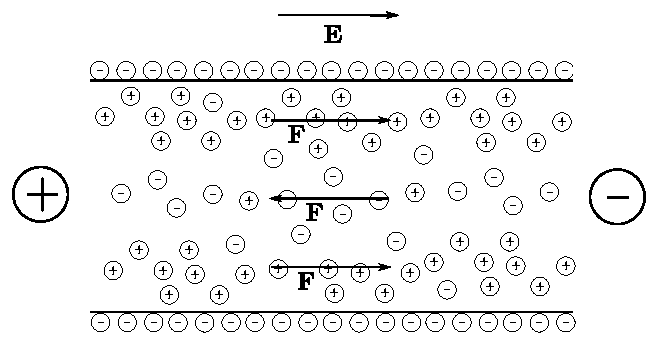
\includegraphics[width=0.7\textwidth]{../fig/channel_electroosmosis.pdf}
\end{center}
\end{figure}

\end{frame}

\begin{frame}{Boundary conditions}
Boundary conditions at (charged) walls, $\Gamma$

\begin{itemize*}
\item Poisson's equation: fixed surface charge, $\sigma$
\begin{equation}\label{eq:et:fix_c}
\nabla\psirm(\x) \cdot \n =
-\frac{\sigma(\x)}{\epsilon_0\epsilon_r}\;,\;\; \x \in \Gamma
\end{equation}

\item Nernst-Planck: zero flux through wall
\begin{equation}\label{eq:et:j0}
\J(\x) \cdot \mathbf{n} = 0 \;,\;\; \x \in \Gamma
\end{equation}

\item Navier-Stokes: no-slip
\begin{equation}
\ubf(\x) = 0 \;,\;\; \x \in \Gamma
\end{equation} 

\end{itemize*}
\end{frame}


\section{The lattice-Boltzmann method}

\subsection{A brief introduction}

\begin{frame}{A few words about the LBM}

\begin{itemize*}

\item Unconventional method to solve PDEs

\item Strengths: complex boundaries, straight-forward implementation,
  highly prallelisable algorithm

\item Weaknesses: New method $\implies$ lack of theoretical work,
  uniform lattice required also Kn $\ll 1$, 


\end{itemize*}

\end{frame}


%\subsection{How}


\section{Some results}

\subsection{Potential and charge distribution}

\begin{frame}{Charge distribution in 2D channel}
Thin channel, no flow, steady state:

\begin{figure}
\begin{center}
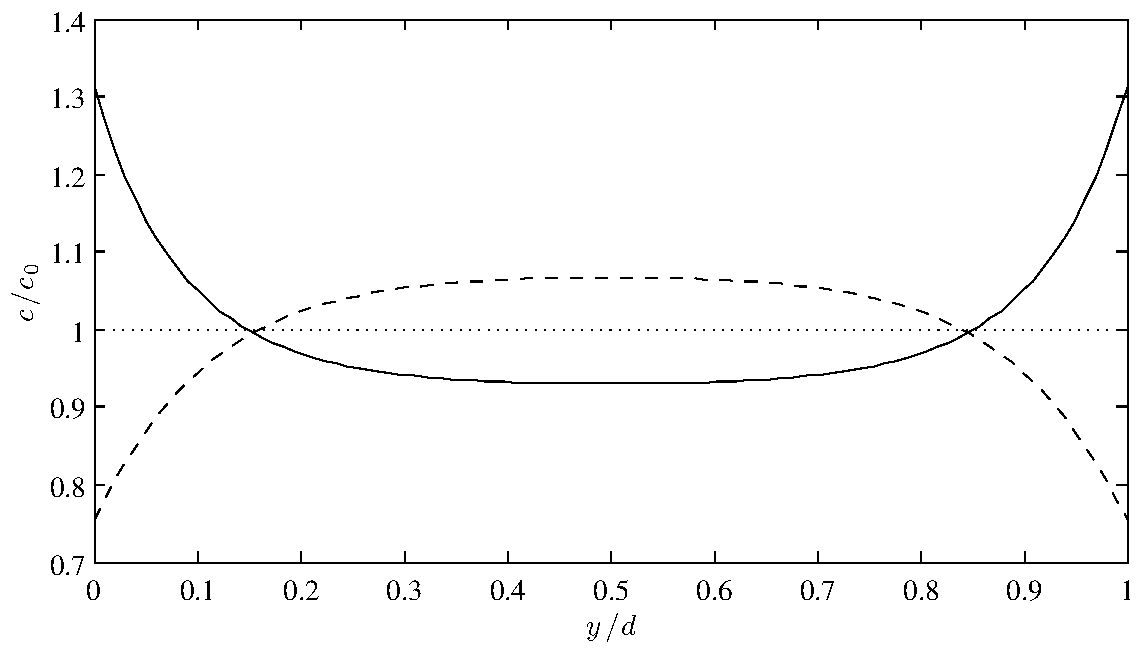
\includegraphics[width=0.9\textwidth]{../fig/charge_1d.pdf}
\end{center}
\caption{Computed positive (solid) and negative (dashed) charge
  distribution across a channel of width $d = 10 \mu$m. The solution
  in the channel is a KCl solution defined by parameters in table
  \ref{tab:res:param}. The channel walls are negatively charged.}
\label{fig:res:c_1d}
\end{figure}

\end{frame}

\subsection{Electroviscous effect}

\begin{frame}{Electroviscous effect in 2D channel}

Flow driven by a pressure gradient, walls of channel charged.

\begin{figure}
\begin{center}
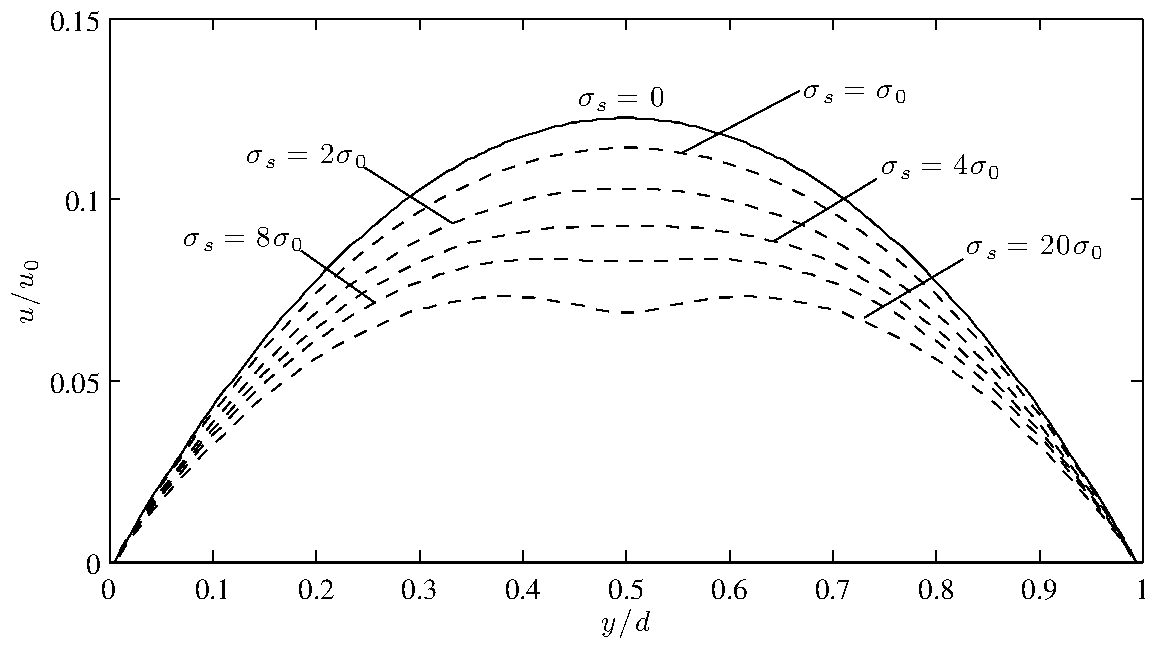
\includegraphics[width=0.9\textwidth]{../fig/electrovisc.pdf}
\end{center}
\caption{Computed velocity profiles across a 2D channel of width $d =
  1 \mu$m. The flow is driven by a pressure gradient and the flow is
  slowed down due to the electroviscouos effect, this effects
  dependence on the surface charge $\sigma_s$ is here illustrated. The
  solution in the channel is a KCl solution defined by parameters in
  table \ref{tab:res:param}. In this simulation, $\sigma_0 = 0.89
  \mu$C/m$^2$, $\partial_xP = 1$ kPa/m and $u_0 = 10$ mm/s. }
\label{fig:res:ev}
\end{figure}
\end{frame}

\begin{frame}{Comparison with ``traditional'' approach}


\begin{figure}
\begin{center}
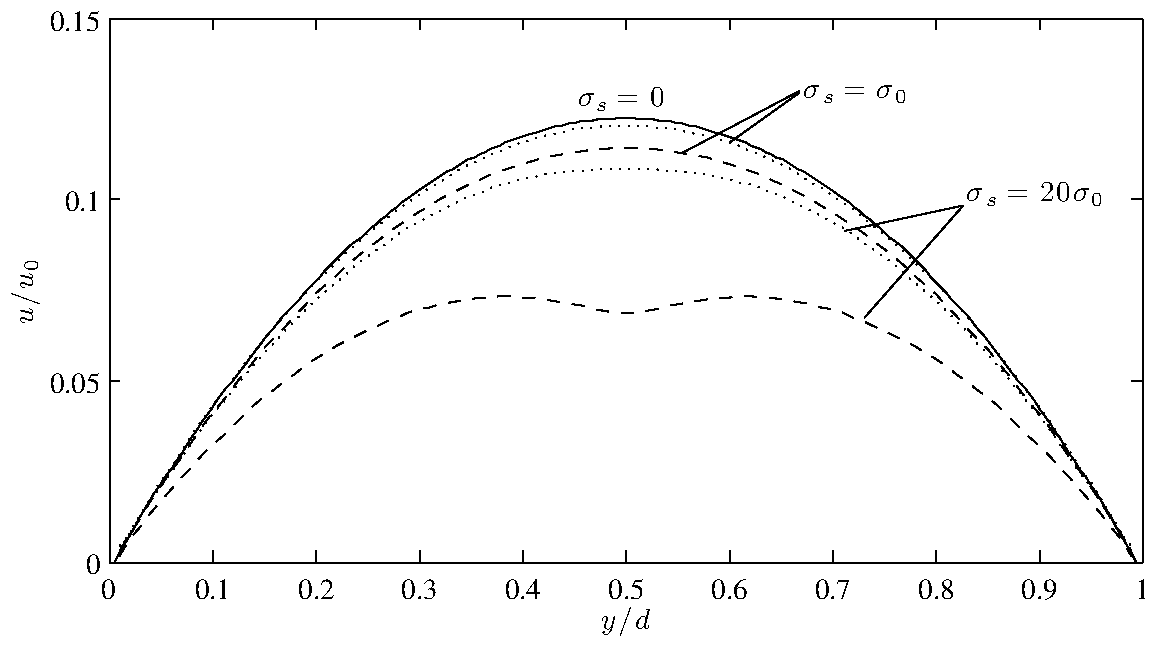
\includegraphics[width=0.9\textwidth]{../fig/electrovisc_comp.pdf}
\end{center}
\caption{Comparison between velocity profiles computed using a mean
  current (dotted) and by using the actual local current (dashed) for
  the streaming potential. The solution in the channel is a KCl
  solution defined by parameters in table \ref{tab:res:param}. In this
  simulation, $\sigma_0 = 0.89 \mu$C/m$^2$, $\partial_xP = 1$ kPa/m
  and $u_0 = 10$ mm/s. }
\label{fig:res:ev_comp}
\end{figure}

\end{frame}

\subsection{Flow through square array}

\begin{frame}{Flow through square array}

\begin{figure}
\begin{center}
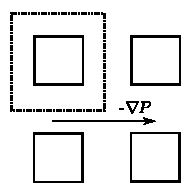
\includegraphics[width=0.7\textwidth]{../fig/square_setup.pdf}
\end{center}

\end{figure}

\end{frame}

\begin{frame}[plain]
\captionsetup[subfloat]{font=normalsize,
labelformat=empty,labelsep=space}

\begin{figure}
  \centering
  \subfloat{\label{fig:res:hedtasdro}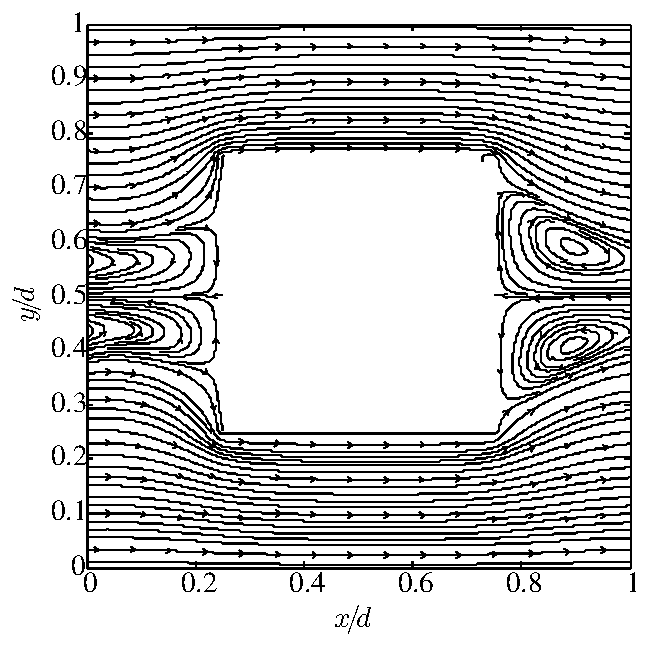
\includegraphics[width=0.40\textwidth]{../fig/s_field_uncharged.pdf}}      
  \hspace{5pt}  \subfloat{\label{fig:resd:asas}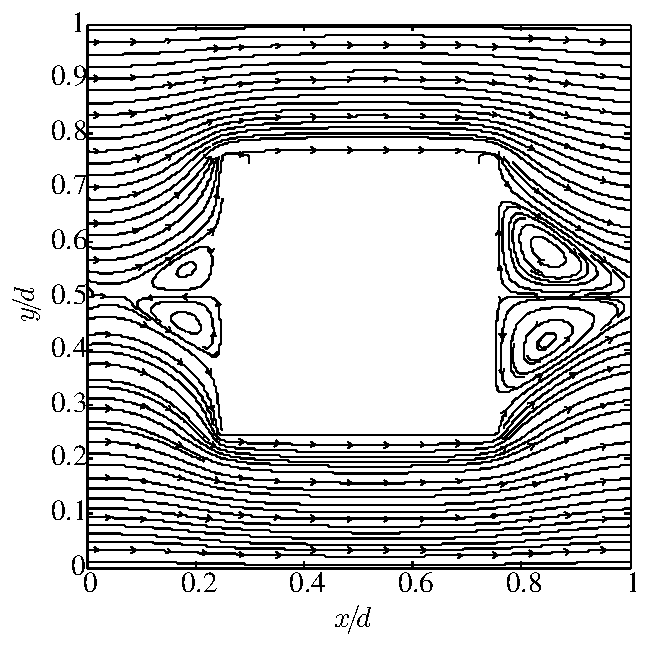
\includegraphics[width=0.40\textwidth]{../fig/s_field_charged.pdf}}
\end{figure}

\vspace{-10pt}

\begin{figure}
  \centering
  \subfloat[$\;\;$ Uncharged
    ]{\label{fig:res:hetasddrdo}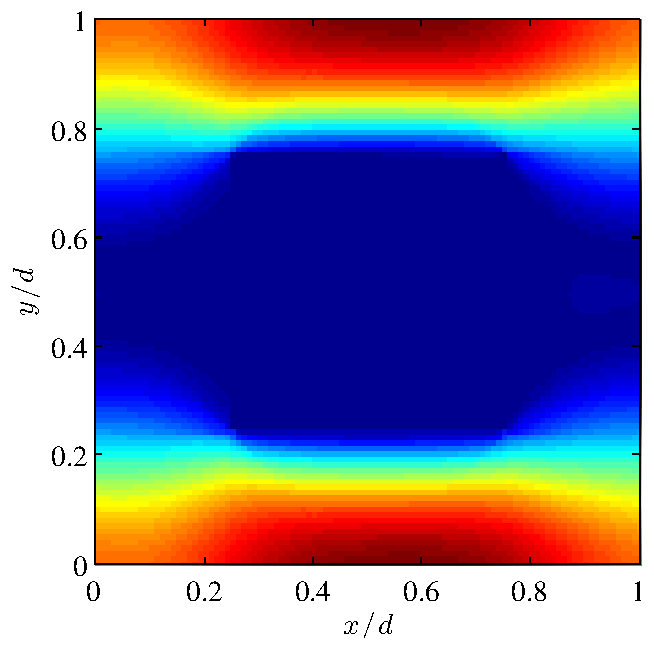
\includegraphics[width=0.40\textwidth]{../fig/s_u_uncharged.pdf}}      
  \hspace{5pt}  \subfloat[$\;\;$ Charged
    ]{\label{fig:res:asdas}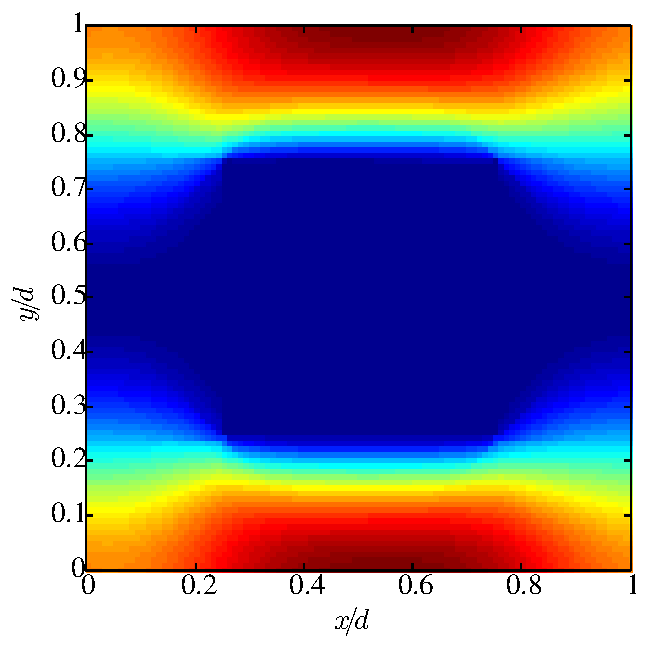
\includegraphics[width=0.40\textwidth]{../fig/s_u_charged.pdf}}
\end{figure}

\end{frame}

\begin{frame}{Flow through square array}

\begin{figure}
\begin{center}
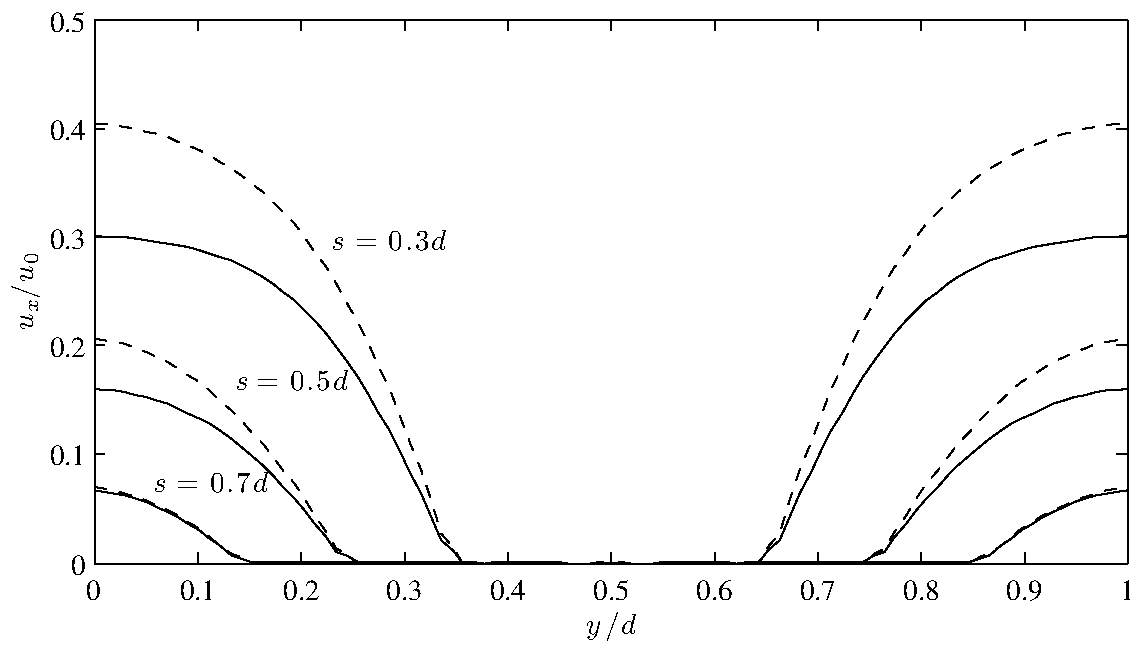
\includegraphics[width=0.9\textwidth]{../fig/square_u_mid.pdf}
\end{center}
\caption{Velocity profiles across the square array at $x = d/2$ in the
  cell. The sides of the squares are varied between $0.3d$, $0.5d$ and
  $0.7d$ where $d = 10 \mu$m is the length of the cell. The flow is
  driven by a pressure gradient and the uncharged (dashed) and charged
  (solid) squares are compared. In this simulation, $\sigma_s = 1.78
  \mu$C/m$^2$ (solid), $\partial_xP = 0.5$ kPa/m and $u_0 = 1$ mm/s. }
\label{fig:res:mid}
\end{figure}

\end{frame}

\section{Conclusions}

\begin{frame}{Main conclusions}

\begin{itemize*}

\item The LBM is a computational alternative in the modelling of
  electrokinetics.

\item The traditional way of computing the streaming potential does
  not give accurate results in thin channels. 

\item Due to the electrovicous effect, the permeability of charged
  structures is decreased.

\end{itemize*}

\end{frame}


\begin{frame}

\begin{center}
\Huge{Thanks for listening!}
\end{center}

\begin{center}
\Huge{Questions?}
\end{center}
\end{frame}


\end{document}



